\documentclass[12pt,a4paper]{article}
\usepackage[utf8]{inputenc}
\usepackage[T1]{fontenc}
\usepackage[brazil]{babel}
\usepackage{amsmath,amssymb}
\usepackage{graphicx}
\usepackage[margin=2.5cm]{geometry}

\begin{document}

\section{Função Massa de Probabilidade (PMF) e Função de Distribuição Acumulada (CDF)}

Considere a variável aleatória discreta $X$, que representa o número de requisições com processamento adicional em um lote de $n = 50$ requisições independentes, com probabilidade individual $p = 0{,}08$, isto é:
\[
X \sim \operatorname{Binomial}(50,\, 0{,}08).
\]

O suporte de $X$ é composto pelos valores inteiros $x \in \{0, 1, 2, \dots, 50\}$. Sua Função Massa de Probabilidade (PMF) e sua Função de Distribuição Acumulada (CDF) são dadas, respectivamente, por:
\[
P(X = x) = \binom{50}{x} (0{,}08)^x (0{,}92)^{50-x}, \qquad F(x) = P(X \le x) = \sum_{k=0}^{x} P(X = k).
\]

Na implementação em R, usando as funções \texttt{dbinom} e \texttt{pbinom} no suporte \texttt{0:50}, verificou-se que a soma de todas as probabilidades da PMF é igual a $1$ e que o último valor da CDF, em $x = 50$, também é igual a $1$.

\subsection{Análise do Gráfico da PMF}

A Figura~\ref{fig:pmf_binomial} mostra o gráfico de hastes verticais da PMF de $X$ para todo o suporte de $0$ a $50$.

\begin{figure}[htbp]
\centering
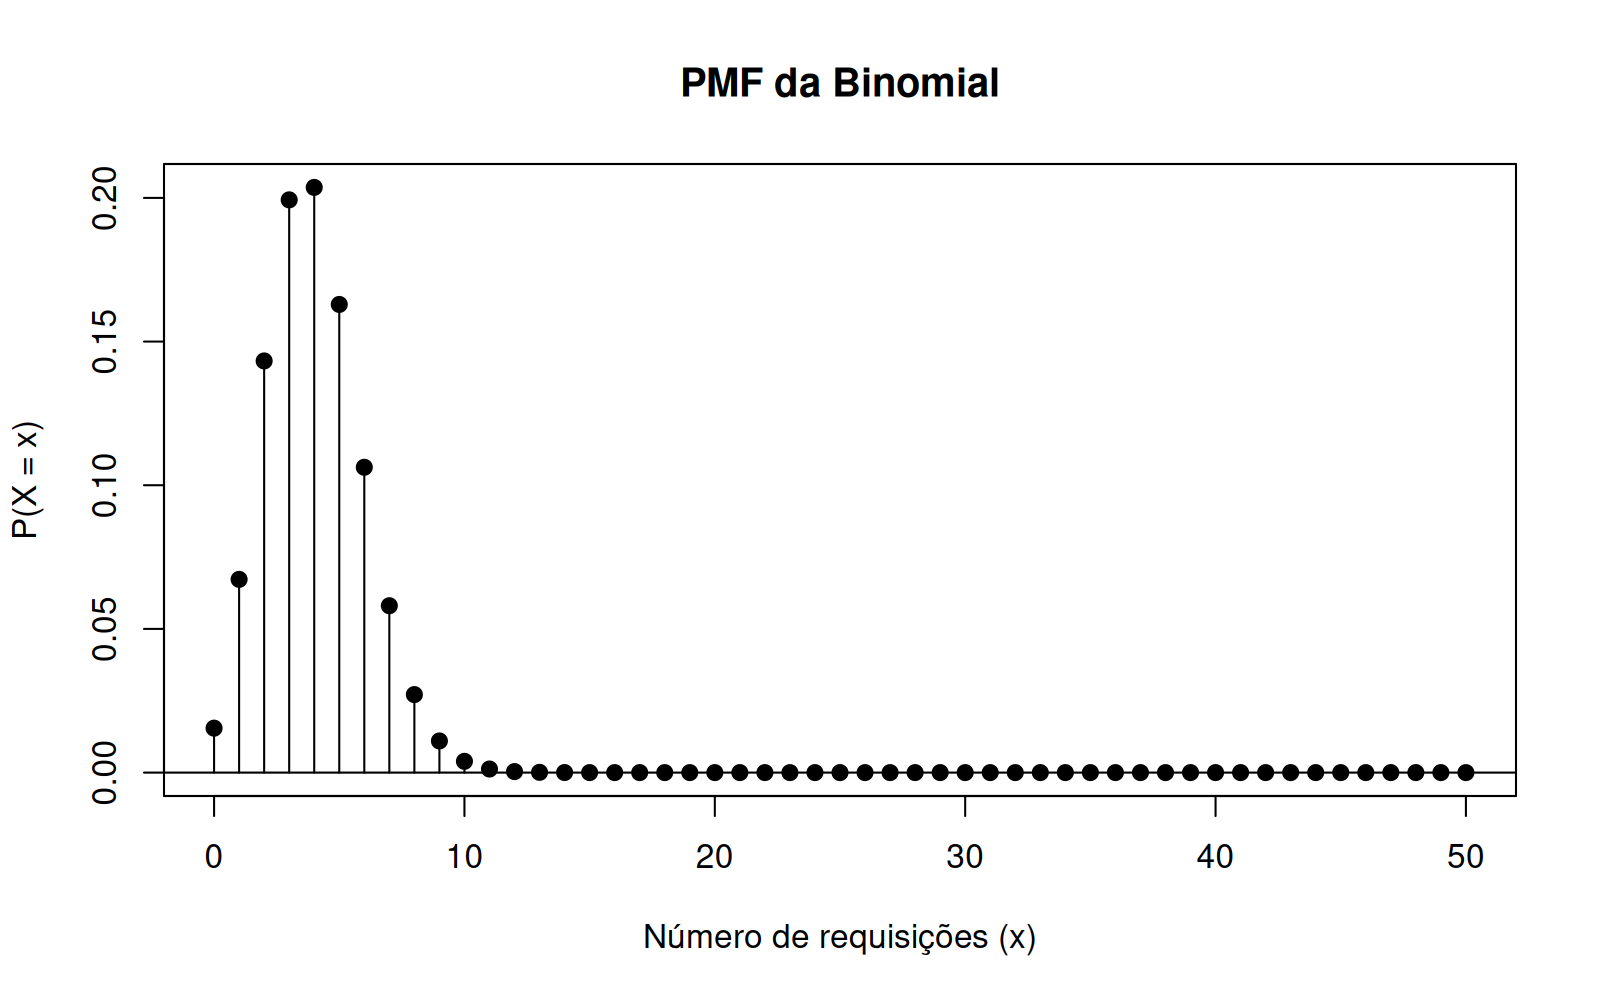
\includegraphics[width=0.85\textwidth]{pmf_binomial.png}
\caption{Função Massa de Probabilidade (PMF) da distribuição $\operatorname{Binomial}(50,\, 0{,}08)$.}
\label{fig:pmf_binomial}
\end{figure}

Pelo gráfico, o ponto mais alto (moda) fica em $x = 4$, com probabilidade $P(X = 4) \approx 0{,}2037$, bem perto de $x = 3$ ($P(X = 3) \approx 0{,}1993$). Também se nota uma \textbf{assimetria positiva} (cauda longa à direita). Isso acontece porque $p = 0{,}08$ é um valor pequeno, então as probabilidades maiores ficam concentradas no início do suporte, perto de $0$, e vão caindo rápido até $50$.

Como a média é $E[X] = 4$ e o desvio padrão é $DP(X) \approx 1{,}92$, a maior parte da probabilidade fica concentrada em volta de $4$. Apenas o intervalo de $x = 2$ até $x = 6$ já soma $P(2 \le X \le 6) \approx 0{,}8154$ (cerca de $81{,}5\%$ do total). Já eventos na cauda direita são muito raros: para $X \ge 15$, tem-se $P(X \ge 15) \approx 5{,}26 \times 10^{-6}$, por isso os pontos a partir de $15$ ficam praticamente colados na linha $y = 0$.

\subsection{Análise do Gráfico da CDF}

A Figura~\ref{fig:cdf_binomial} mostra o gráfico em escada da CDF de $X$, representando a probabilidade acumulada $F(x) = P(X \le x)$ entre $0$ e $1$.

\begin{figure}[htbp]
\centering
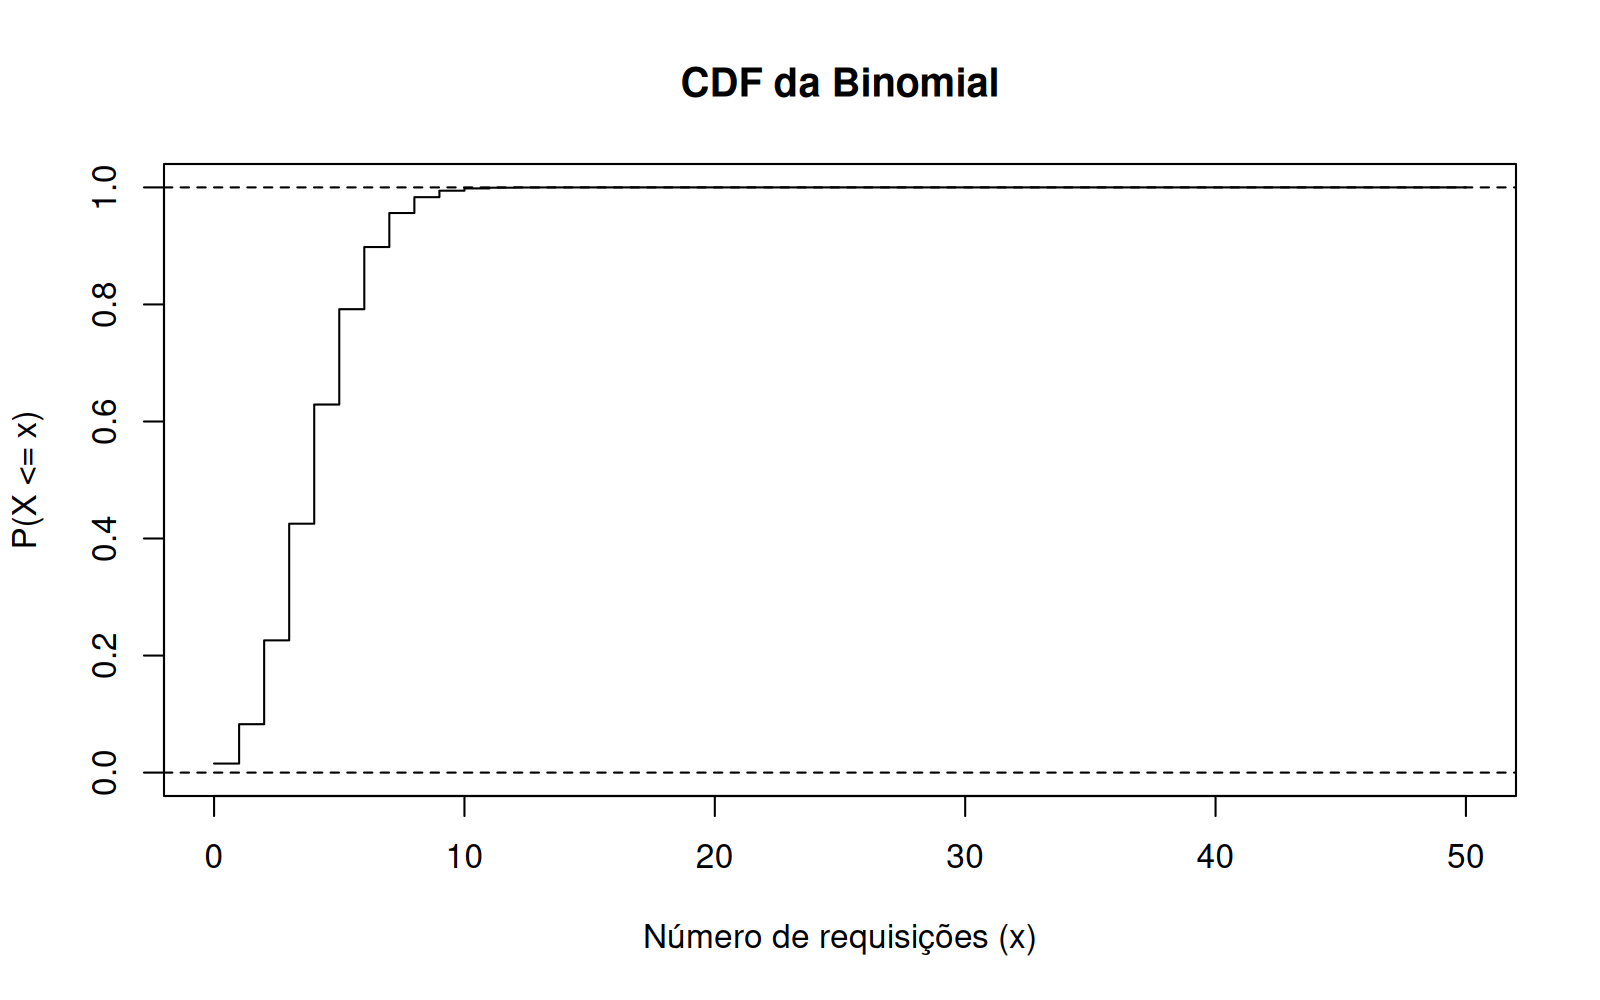
\includegraphics[width=0.85\textwidth]{cdf_binomial.png}
\caption{Função de Distribuição Acumulada (CDF) da distribuição $\operatorname{Binomial}(50,\, 0{,}08)$.}
\label{fig:cdf_binomial}
\end{figure}

Como $X$ é uma variável discreta, a CDF cresce em degraus, e a altura de cada salto em $x$ corresponde exatamente ao valor da PMF naquele ponto. Por isso, os degraus são bem altos entre $x = 2$ e $x = 6$, que é onde a PMF tem os maiores valores: nesse trecho, o acumulado sobe de $F(2) \approx 0{,}2260$ até $F(6) \approx 0{,}8981$.

A partir de $x = 10$ ($F(10) \approx 0{,}9983$), os degraus ficam bem pequenos e a curva praticamente achata na linha $y = 1$ muito antes de chegar em $x = 50$. Em $x = 15$, por exemplo, a probabilidade acumulada já chega a $F(15) \approx 0{,}999999$.

\end{document}
